\documentclass[dvipsnames,svgnames]{beamer}

\usepackage{epsfig}
\usepackage{float}
\usepackage{subfigure}
\usepackage{url}
\usepackage{graphicx}
\usepackage{alltt}
\usepackage{color}
\usepackage{verbatim}

\renewcommand{\phi}{\varphi}

\usepackage{lipsum}
\newcommand\blfootnote[1]{%
  \begingroup
  \renewcommand\thefootnote{}\footnote{#1}%
  \addtocounter{footnote}{-1}%
  \endgroup
}

\usetheme{KYRsplit}
\usetheme{Darmstadt}

\newcommand{\pspic}[2]{\scalebox{#1}{\includegraphics{#2}}}

\setbeamercovered{transparent}

\setbeamersize{text margin right = 0.5cm}
\setbeamersize{text margin left = 0.5cm}

\title[NSF:CCRI TAB Meeting]{NSF:CCRI: Developing an Open-Source, State-of-the-Art Symbolic Model-Checking Framework for the Model-Checking Research Community}
\author{Rozier, Shankar, Tinelli, Vardi}
\date{November 8 \& December 6, 2021}

\begin{document}

\begin{frame}[fragile]  
  \huge
  \begin{center}
    \setbeamercolor{KYRatitle}{fg=white, bg=\structure{}}
    \begin{beamercolorbox}[center]{title}

      \inserttitle

      \medskip
    \end{beamercolorbox}

    \normalsize
    
    \medskip
    {\large Rozier, Shankar, Tinelli, Vardi}
        \vspace{0.2in}

        \centerline{ \structure{\Large \bf Technical Advisory Board Meeting}}
        
     {\large November 8 \& December 6, 2021}

    \bigskip
 

\centerline{Website Coming Soon\ldots}
\centerline{\textcolor{red}{\url{ https://www.aere.iastate.edu/modelchecker/}}}
  \end{center}
\end{frame}


\section{About}
\subsection{ } %make the dots appear at the top


\begin{frame}
\frametitle{The Problem\footnote{\tiny K.Y.Rozier and M.Y.Vardi, ``A Multi-Encoding Approach for LTL Symbolic Satisfiability Checking,'' FM 2011.}}

\vspace{-0.1in}
    \begin{center}
      \pspic{0.32}{figs/R2scaleableRunTime_logscale-eps-converted-to.pdf} \\

\normalsize
    \end{center}

\end{frame}

\begin{frame}
\frametitle{FuseIC3: An Algorithm for Checking Large Design Spaces\footnote{\tiny{Rohit Dureja and Kristin Yvonne Rozier. ``FuseIC3: An Algorithm for Checking Large Design Spaces.'' In Formal Methods in Computer-Aided Design (FMCAD), IEEE/ACM, Vienna, Austria, October 2-6, 2017.}}}

\vspace{-0.1in}
\centering
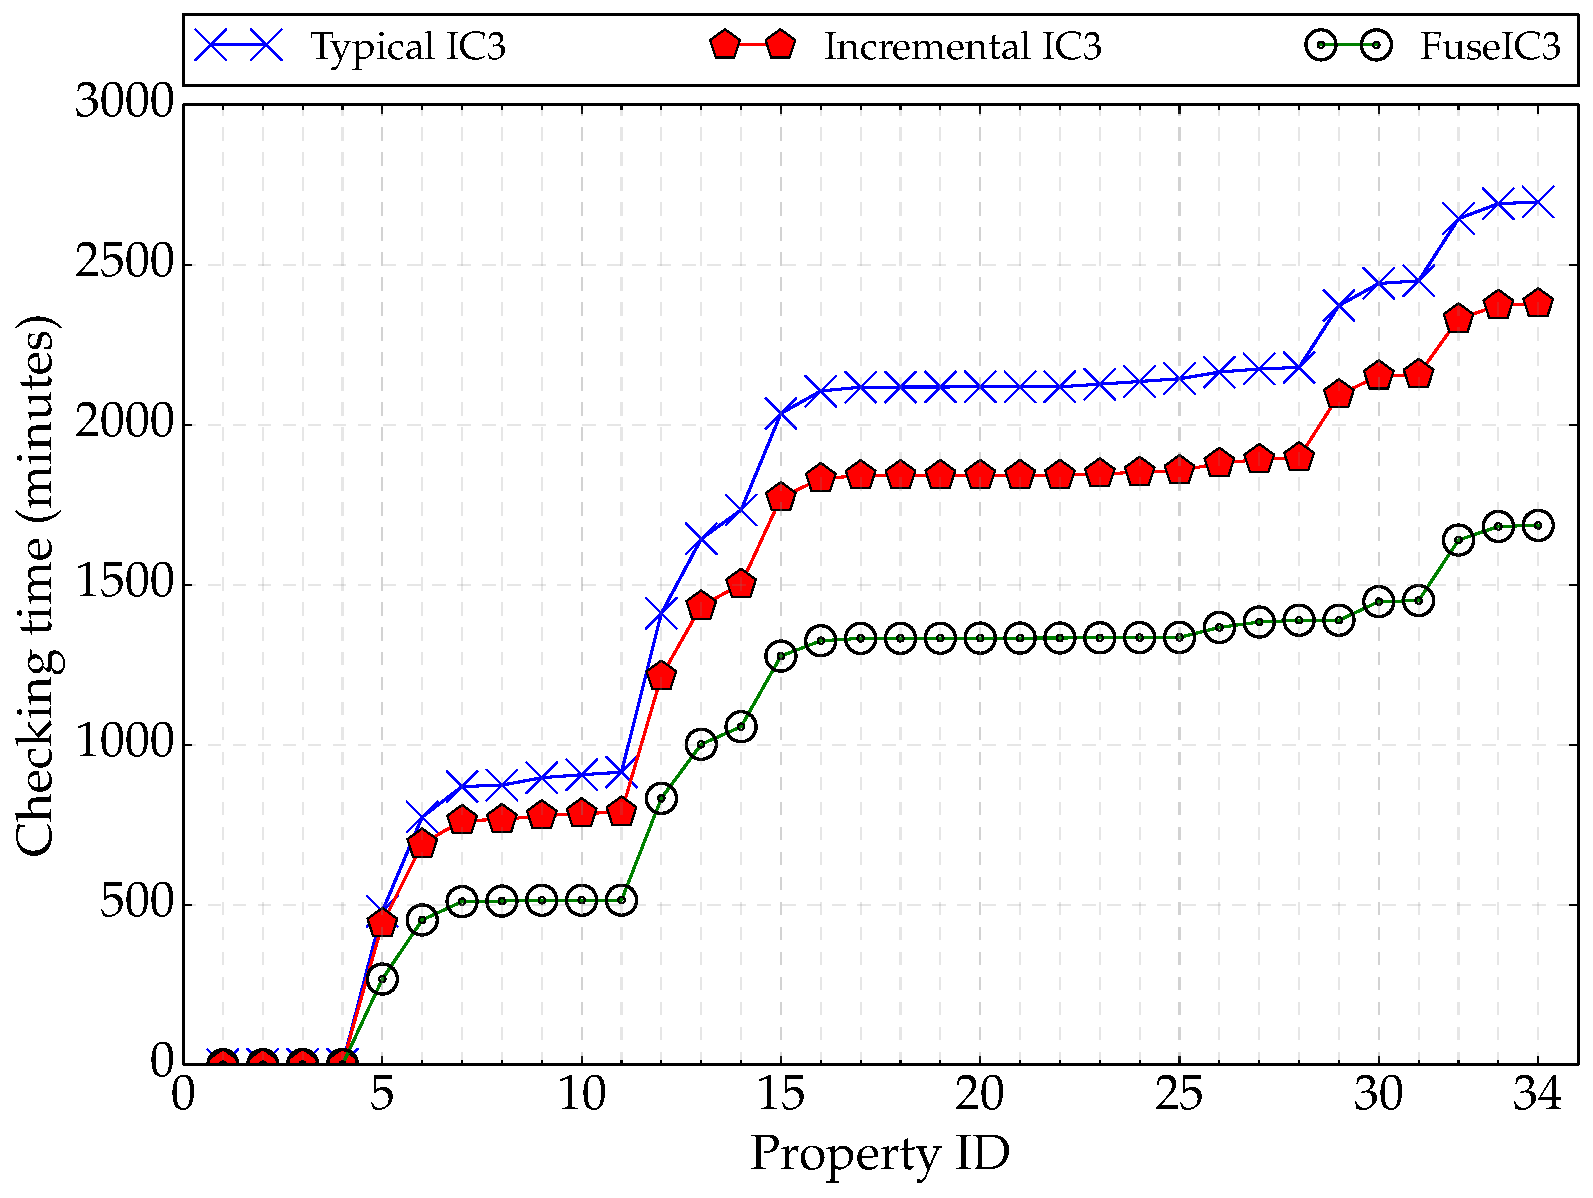
\includegraphics[height=0.75\textheight]{figs/heuristics_time.pdf}\\
Model checking \textcolor{OliveGreen}{\bf 34 formulas} over \textcolor{RedViolet}{\bf 1,620 models} is \textcolor{red}{\bf 5.48x faster}

\end{frame}


\begin{frame}
\frametitle{The Problem Continues\ldots}


\begin{itemize}
\item nuXmv, CadenceSMV, others are \textcolor{red}{\bf closed source} \\ \ \\
\item ABC, HWMCC tools are \textcolor{RedViolet}{\bf limited to low-level modeling languages} \\ \ \\
\item No \textcolor{OliveGreen}{\bf open-source, research-enabling connection} between:
  \begin{itemize}
  \item Rich modeling languages with real-world benchmark models
  \item State-of-the-art back-end MC algorithms
\end{itemize}
\end{itemize}

\end{frame}




\begin{frame}

  \begin{center}
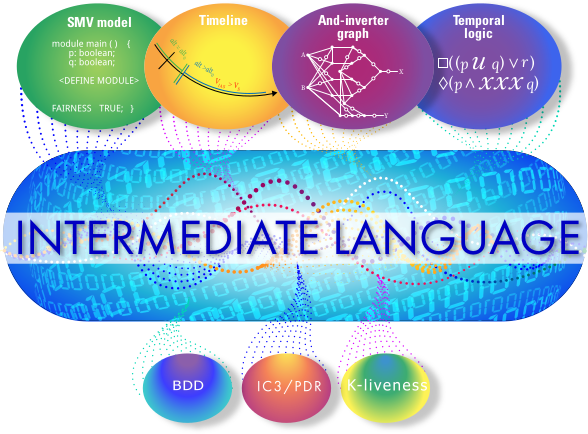
\includegraphics[height=\textheight]{figs/IntermediateLanguageFig.pdf}
\end{center}

\end{frame}


\begin{frame}
  \frametitle{Goals for Intermediate Language}

  \begin{itemize}
\item Allow adding a \textcolor{RedViolet}{\bf modeling language} via \textcolor{MidnightBlue}{\bf translation to/from IL} \\ \ \\
\item Allow adding an \textcolor{RedViolet}{\bf MC algorithm} via \textcolor{MidnightBlue}{\bf translation to/from IL}  \\ \ \\
\item IL is efficient/accessible so as to \textcolor{OliveGreen}{\bf encourage usage in future MCs}  \\ \ \\
\item IL suitable for on-going \structure{\bf community standard}

    \end{itemize}

  \end{frame}


\begin{frame}
\frametitle{Agenda}

\begin{enumerate}
\item Goals \& objectives overview (questions?) \\ \ \\
\item Initial proposal for a community model checking intermediate language \\ \ \\
  \item Moderated discussion
\end{enumerate}

\end{frame}

\end{document}
